A documentação da \acrshort{api} de dados é bastante importante por forma a ajudar futuros programadores e
utilizadores a usarem a plataforma da \acrshort{clav}.

Para proceder à documentação em \textit{Swagger} da \acrshort{api} de dados da \acrshort{clav} é essencial
perceber o que é o \textit{Swagger} (\textit{OpenAPI} e \textit{Swagger UI}) e suas alternativas.
Isto é observado no estado da arte que se apresenta a seguir.

\section{Estado da Arte}

\subsection{Swagger}
O \textit{Swagger} é um ecossistema de ferramentas para desenvolver \acrshort{api}s com a \acrfull{oas}.

Até 2015 o \textit{Swagger} consistia numa especificação e num ecossistema de ferramentas para implementar a 
especificação. Em 2015 a fundadora do \textit{Swagger}, \textit{SmartBear Software}, doou a especificação 
\textit{Swagger} para a \textit{Linux Foundation} e renomeou a especificação para \acrlong{oas}.~\cite{wiswagger}

A especificação \textit{OpenAPI} é agora desenvolvida pela \textit{OpenAPI Initiative} que envolve várias 
empresas tecnológicas entre as quais \textit{Microsoft}, \textit{Google}, \textit{IBM} e a 
fundadora \textit{Smartbear Software}.

Já o conjunto de ferramentas \textit{Swagger} inclui ferramentas \textit{open-source}, gratuitas e comerciais 
que podem ser usadas em diferentes estágios do ciclo de vida de uma \acrshort{api}, que inclui documentação, 
desenho, testes e \textit{deployment}. Algumas das ferramentas são:~\cite{swaggerVSoas}
\begin{itemize}
    \item \textbf{\textit{Swagger Editor}}: Permite editar especificações \textit{OpenAPI} em 
    \acrshort{yaml} no \textit{browser}\footnote{Aceder \url{https://editor.swagger.io/}}, 
    validar as especificações em relação às regras do \acrshort{oas} bem como pré-visualizar 
    a documentação em tempo real. Facilita o desenho e a documentação de \acrshort{api}s \acrshort{rest};

    \item \textbf{\textit{Swagger \acrshort{ui}}}: Coleção de \textit{assets} \textit{\acrshort{html}}, 
    \textit{JavaScript} e \textit{\acrshort{css}} que geram dinamicamente documentação a partir de uma 
    especificação \textit{OpenAPI} de uma \acrshort{api};

    \item \textbf{\textit{Swagger Codegen}}: Permite a geração de bibliotecas cliente (geração de \acrshort{sdk}), 
    \textit{server stubs} e documentação automática a partir de especificações \textit{OpenAPI};

    \item \textbf{\textit{Swagger Inspector}}: Ferramenta de testes de \acrshort{api}s que permite validar 
    as \acrshort{api}s e gerar definições \textit{OpenAPI} de \acrshort{api}s existentes;

    \item \textbf{\textit{SwaggerHub}}: Desenho e documentação de \acrshort{api}s, construído para equipas que 
    trabalham com \textit{OpenAPI}.
\end{itemize}

O \textit{Swagger} possui duas abordagens:~\cite{swaggerNode}
\begin{itemize}
    \item \textit{top-down}: Uso do \textit{Swagger Editor} para criar a especificação \textit{OpenAPI} e 
    depois usar o \textit{Swagger Codegen} por forma a gerar o código do cliente e do servidor. Ou seja, 
    primeiro desenha-se a \acrshort{api} antes de escrever código;

    \item \textit{bottom-up}: Utilizador já possui uma \acrshort{api} \acrshort{rest} e o \textit{Swagger} irá 
    ser usado apenas para documentar a \acrshort{api} existente.
\end{itemize}

Visto que a \acrshort{clav} já possui grande parte da \acrshort{api} construída vai ser usada uma abordagem 
\textit{bottom-up}. Portanto, o \textit{Swagger} vai ser usado apenas para a documentação da \acrshort{api}. 
De forma a produzir a documentação, do portfólio de ferramentas do \textit{Swagger} apenas precisaremos de 
utilizar o \textit{Swagger \acrshort{ui}} e o \textit{Swagger Editor}. O primeiro permitirá apresentar aos 
utilizadores a documentação gerada e o segundo permitirá validar a especificação \textit{OpenAPI} (documentação) 
criada, verificando se não possui erros.

\subsection{Especificação \textit{OpenAPI}}

A especificação \textit{OpenAPI} providencia um conjunto de propriedades que podem ser usadas para descrever 
uma \acrshort{api} \acrshort{rest}. Com um documento de especificação válido é possível usá-lo para criar uma 
documentação interativa, por exemplo, através do \textit{Swagger \acrshort{ui}}.

De seguida será apresentado o que é possível documentar com a especificação \textit{OpenAPI} e como. 
É possível usar tanto \acrshort{yaml} como \acrshort{json} para a especificar. Esta parte será demonstrada 
usando \acrshort{yaml}.\footnote{A especificação completa do \textit{OpenAPI} com versão igual a 3.0.0 pode 
ser vista em \url{https://github.com/OAI/OpenAPI-Specification/blob/master/versions/3.0.0.md}}

\subsubsection{Metadata}
O primeiro passo é escolher a versão da especificação \textit{OpenAPI} que irá ser usada para documentar:
\begin{lstlisting}[language=yaml, caption=Exemplo de indicação da versão da especificação \textit{OpenAPI}]
openapi: 3.0.0
\end{lstlisting}

Depois, na secção \texttt{info}, é possível descrever um pouco a \acrshort{api} que estamos a documentar, 
indicando o título, a descrição e a versão da mesma. As propriedades \texttt{title} e \texttt{version} são 
obrigatórias. É possível também colocar informação sobre os contactos disponíveis, termos de uso e a 
licença:\footnote{Ver mais em \url{https://github.com/OAI/OpenAPI-Specification/blob/master/versions/3.0.0.md\#infoObject}}
\begin{lstlisting}[language=yaml, caption={Exemplo de secção \texttt{info} indicando título, descrição e versão da \acrshort{api} na especificação \textit{OpenAPI}}]
info:
  title: CLAV API
  description: Esta é a API do projeto CLAV...
  version: 1.0.0
\end{lstlisting}

\vspace{-0.7cm}

\subsubsection{Servidores}
Há depois uma secção com o nome de \texttt{servers} para indicar os \textit{URL}s que são os pontos de acesso 
da \acrshort{api}. Podem ser indicados vários pontos de 
acesso:\footnote{Para mais detalhes sobre esta secção veja \url{https://swagger.io/docs/specification/api-host-and-base-path/}}
\begin{lstlisting}[language=yaml, caption=Exemplo de secção \texttt{servers} indicando os \textit{URL}s e a descrição de cada na especificação \textit{OpenAPI}]
servers:
  - url: http://clav-api.dglab.gov.pt/api
    description: Official API server
  - url: http://clav-test.di.uminho.pt/api
    description: Testing server
  - url: http://localhost:7779/api
    description: Local server
\end{lstlisting}

\vspace{-0.7cm}

\subsubsection{Caminhos/Rotas}
De seguida apresenta-se uma das secções mais importantes da especificação, a secção \texttt{paths}. 
Aqui são definidas as rotas que a \acrshort{api} disponibiliza. Para definir cada rota basta indicar o caminho 
relativo aos pontos de acesso definidos na secção \texttt{servers} (\verb|<server-url>/<caminho relativo>|). 
Nesta secção é definido tudo o que envolve as rotas, desde os parâmetros necessários, as respostas que devolve, 
os métodos \textit{HTTP} disponíveis, etc:\footnote{Mais detalhes em \url{https://swagger.io/docs/specification/paths-and-operations/}}\footnote{mais detalhes sobre a funcionalidade \texttt{\$ref} em \url{https://swagger.io/docs/specification/using-ref/}}
\begin{lstlisting}[language=yaml, caption=Exemplo de secção \texttt{paths} indicando os detalhes de cada rota na especificação \textit{OpenAPI}, label={exem:oapiRota}]
paths:
  /users/{id}:
    get:
      summary: Resumo do que faz a rota
      description: >
        Descrição detalhada, pode ser usado Markdown para enriquecer o texto
      parameters:
        - name: id
          in: path
          description: Id do utilizador
          required: true
          schema:
            type: string
      responses:
        200:
          description: Descrição da resposta, p.e: Sucesso
          content:
            application/json:
              schema:
                #A estrutura do JSON devolvido pode ser definido logo aqui ou num componente à parte, fazendo referência desse. Iremos aplicar o segundo caso para demonstrar que estas funcionalidades tornam a documentação mais fácil de manter
                $ref: '#/components/schemas/User'
        ...
    post:
      ...
    delete:
      ...
  /users:
    ...

components:
  schemas:
    User:
      type: object
      properties:
        id:
          type: string
        ...
      required:
        - id
        ...
\end{lstlisting}

Outro ponto importante a referir é que é possível agrupar as rotas em grupos através do uso de \textit{tags}. 
As \textit{tags} têm de ser definidas numa secção chamada \textit{tags}:
\begin{lstlisting}[language=yaml, caption={Exemplo de secção \texttt{tags} definindo tags na especificação \textit{OpenAPI}}]
tags:
  - name: users
    description: Descrição
  - name: classes
    description: Outra descrição
\end{lstlisting}

Depois em cada rota é necessário indicar a que \textit{tag} (grupo) pertence:
\begin{lstlisting}[language=yaml, caption=Exemplo de uso de \textit{tags} numa rota na especificação \textit{OpenAPI}]
paths:
  /users/{id}:
    get:
      summary: Resumo do que faz a rota
      tags:
        - users
      ...
\end{lstlisting}

\vspace{-0.7cm}

\subsubsection{Parâmetros}\label{sec:paramSwagger}
Como já exemplificado no exemplo~\ref{exem:oapiRota} os parâmetros de uma rota são definidos na 
secção \texttt{parameters} de cada rota. 
Existem quatro tipo de parâmetros que variam de acordo com o local onde se encontram. 
O tipo de um parâmetro é definido na propriedade \texttt{in} de um parâmetro e pode ser um dos seguintes:
\begin{itemize}
    \item Parâmetros no caminho: Servem normalmente para apontar para um recurso específico. 
    Estes parâmetros são sempre obrigatórios como tal a propriedade \texttt{required} com o valor igual a 
    verdadeiro deve ser sempre adicionada. Para além disso o \texttt{name} tem de ser igual ao que está no 
    caminho. A propriedade \texttt{in} tem o valor de \textit{path};
    \item Parâmetros na \textit{query string}: A propriedade \texttt{in} tem o valor de \textit{query}. 
    No caso de tokens passados em parâmetros da \textit{query string} devem-se usar esquemas de segurança, 
    veja a secção~\ref{sec:authSwagger};
    \item Parâmetros no cabeçalho: A propriedade \texttt{in} tem o valor de \textit{header}. 
    Contudo os cabeçalhos \textit{Accept}, \textit{Content-Type} e \textit{Authorization} não são aqui definidos;
    \item Parâmetros no cabeçalho da \textit{Cookie}: A propriedade \texttt{in} tem o valor de \textit{cookie}.
\end{itemize}

Cada parâmetro tem várias propriedades que permitem defini-lo:\footnote{Mais detalhes em \url{https://swagger.io/docs/specification/describing-parameters/}}
\begin{itemize}
    \item \texttt{required}: Indica se o parâmetro é obrigatório ou opcional. 
    Possíveis valores são \textit{true} ou \textit{false}.
    \item \texttt{schema}:
    \begin{itemize}
        \item \texttt{default}: Valor padrão de um parâmetro opcional;
        \item \texttt{type}: O tipo do parâmetro. Possíveis valores: \textit{string}, \textit{integer}, etc;
        \item \texttt{enum}: Indica os possíveis valores para o parâmetro;
        \item \texttt{nullable}: Indica se o parâmetro pode ser \textit{null}. Possíveis valores são 
        \textit{true} ou \textit{false}.
    \end{itemize}
    \item \texttt{allowEmptyValue}: Indica se o parâmetro pode ser vazio. Apenas aplicável no caso de um 
    parâmetro na \textit{query string}. Possíveis valores são \textit{true} ou \textit{false};
    \item \texttt{example}: Um exemplo do valor;
    \item \texttt{examples}: Múltiplos exemplos;
    \item \texttt{deprecated}: Indica se o parâmetro é ou não \textit{deprecated}. Possíveis valores são 
    \textit{true} ou \textit{false}.
\end{itemize}

\subsubsection{\textit{Request Body}}
O \textit{request body} é definido em cada rota na secção \texttt{requestBody} sendo usado essencialmente em 
rotas com o método \acrshort{http} igual a POST ou a PUT, ou seja, em casos que há necessidade de criar ou alterar 
um objeto de acordo com a informação fornecida no pedido. As propriedades que podem ser definidas no 
\texttt{requestBody} são as seguintes:\footnote{Para mais detalhes, desde \textit{upload} de ficheiros, a \textit{Form Data}s, veja em \url{https://swagger.io/docs/specification/describing-request-body/}}\footnote{Para mais informação sobre os \textit{media types} veja \url{https://swagger.io/docs/specification/media-types/}}
\begin{itemize}
    \item \texttt{description}: Opcionalmente pode ser adicionada uma descrição;
    \item \texttt{required}: Indica se o \textit{request body} é obrigatório ou opcional. 
    Possíveis valores são \textit{true} ou \textit{false}. Por omissão o \textit{request body} é opcional;
    \item \texttt{content}: Obrigatório. Lista os \textit{media types} consumidos pela rota e especifica 
    o \texttt{schema} para cada \textit{media type}.
\end{itemize}

\subsubsection{Respostas}
Nesta secção, propriedade \texttt{responses} de cada rota, é descrita as possíveis respostas de cada rota. 
Na propriedade serão definidas as várias respostas, uma resposta por cada \acrshort{http} \textit{status code} 
possível de ser devolvido pela rota. Cada resposta pode possuir as seguintes propriedades:\footnote{Mais detalhes em \url{https://swagger.io/docs/specification/describing-responses/}}
\begin{itemize}
    \item \texttt{description}: Obrigatório, descrição da resposta;
    \item \texttt{content}: Opcional, semelhante ao \texttt{content} do \textit{request body} e define o 
    conteúdo que é devolvido;
    \item \texttt{headers}: Opcional, define as \textit{headers} que são devolvidas na resposta.
\end{itemize}

\subsubsection{Adição de Exemplos}
Na secção~\ref{sec:paramSwagger} já se referiu como é possível adicionar exemplos aos parâmetros. 
De forma semelhante o mesmo pode ser realizado tanto no \textit{request body} como nas respostas através da 
propriedade \texttt{example} (um exemplo) ou \texttt{examples} (múltiplos exemplos) aninhado(s) na propriedade 
\texttt{schema} ou aninhado(s) na ``propriedade'' \textit{media type} no caso do \texttt{schema} ser uma 
referência para um modelo presente na secção \texttt{components}. A propriedade \texttt{example} pode também ser 
usada em objetos ou propriedades de um \texttt{schema}. Por fim, para adicionar exemplos de \acrshort{xml} ou 
\acrshort{html} os exemplos devem ser \textit{strings}:\footnote{Mais detalhes em \url{https://swagger.io/docs/specification/adding-examples/}}
\begin{lstlisting}[language=yaml, caption=Exemplo de adição de exemplos para \acrshort{xml} e \acrshort{html} na especificação \textit{OpenAPI}]
content:
  application/xml:
    schema:
      $ref: '#/components/schemas/xml'
    examples:
      xml:
        summary: A sample XML response
        value: '<objects><object><id>1</id><name>new</name></object><object><id>2</id></object></objects>'
  text/html:
    schema:
      type: string
      examples:
        html:
          summary: A list containing two items
          value: '<html><body><ul><li>item 1</li><li>item 2</li></ul></body></html>'
\end{lstlisting}

\vspace{-0.7cm}

\subsubsection{Modelos}
A secção \texttt{schemas} presente na secção \texttt{components} permite definir estruturas de dados 
(modelo) a serem usados na \acrshort{api}. 
Estes modelos podem ser referenciados usando a funcionalidade \texttt{\$ref}.\footnote{Mais detalhes em \url{https://swagger.io/docs/specification/data-models/}}

\subsubsection{Autenticação e Autorização}\label{sec:authSwagger}
Nesta secção será demonstrada como se pode adicionar a autenticação e autorização à especificação \textit{OpenAPI}. 
Para tal é necessário criar \textit{security scheme}s. Os esquemas são definidos na secção 
\texttt{securitySchemes} dentro da secção \texttt{components}. 
Para cada esquema de segurança é necessário definir a propriedade \texttt{type}. 
Na especificação é possível descrever os seguintes esquemas de segurança:
\begin{itemize}
    \item Esquemas de autenticação \acrshort{http} (usam o cabeçalho \textit{Authorization}) (\texttt{type} = \texttt{http}):
    \begin{itemize}
        \item \textit{Basic} (propriedade \texttt{scheme} = \texttt{basic});
        \item \textit{Bearer} (propriedade \texttt{scheme} = \texttt{bearer});
        \item Outros esquemas \acrshort{http} definidos pelo \href{https://tools.ietf.org/html/rfc7235}{RFC 7235} 
        e pelo registo de esquemas de autenticação \acrshort{http}.
    \end{itemize}
    \item Chaves \acrshort{api} no cabeçalho, na \textit{query string} ou em \textit{cookies} 
    (\texttt{type} = \texttt{apiKey} e na propriedade \texttt{in} indicar em que local se encontra, se no 
    cabeçalho (\texttt{header}), se na \textit{query string} (\texttt{query}) ou se nas \textit{cookies} 
    (\texttt{cookie}));
    \item \textit{OAuth 2} (\texttt{type} = \texttt{oauth2});
    \item \textit{OpenID Connect Discovery} (\texttt{type} = \texttt{openIdConnect}).
\end{itemize}

Após definir os esquemas de segurança é necessário aplicá-los nas rotas que devem estar protegidas 
por esses esquemas. Para tal em cada rota pode ser definida a propriedade \texttt{security} e indicar 
os esquemas de segurança que essa rota 
suporta.\footnote{Mais detalhes em \url{https://swagger.io/docs/specification/authentication/}}

\subsubsection{Alternativas}
Em termos de alternativas à especificação \textit{OpenAPI} existem duas 
concorrentes: \textit{\acrshort{raml}}\footnote{Ver \url{https://github.com/raml-org/raml-spec/blob/master/versions/raml-10/raml-10.md/}} e \textit{\acrshort{api} Blueprint}\footnote{Ver \url{https://github.com/apiaryio/api-blueprint/blob/master/API\%20Blueprint\%20Specification.md}}.

Comparemos as três hipóteses:~\cite{specsComp}
\begin{table}[H]
    \footnotesize
    \centering
    \begin{tabular}{|r|p{0.385\textwidth}|p{0.385\textwidth}|}
    \hline
    Especificação & Vantagens & Desvantagens \\ \hline
    \textit{OpenAPI} &
        \begin{itemize}[leftmargin=0.3cm, topsep=0cm]
            \setlength\itemsep{0em}
            \item Grande adoção
            \item Grande comunidade de utilizadores
            \item Bom suporte
            \item Suporte para várias linguagens
        \end{itemize}
        &
        \begin{itemize}[leftmargin=0.3cm, topsep=0cm]
            \setlength\itemsep{0em}
            \item Falta de construtores avançados para metadados
        \end{itemize}
        \\ \hline
    \acrshort{raml} &
        \begin{itemize}[leftmargin=0.3cm, topsep=0cm]
            \setlength\itemsep{0em}
            \item Suporta construções avançadas
            \item Adoção decente
            \item \textit{Human readable format}
            \item Grande apoio da indústria 
        \end{itemize}
        &
        \begin{itemize}[leftmargin=0.3cm, topsep=0cm]
            \setlength\itemsep{0em}
            \item Falta de ferramentas ao nível do código
            \item Ainda não comprovado a longo prazo
        \end{itemize}
        \\ \hline
    \textit{\acrshort{api} Blueprint} &
        \begin{itemize}[leftmargin=0.3cm, topsep=0cm]
            \setlength\itemsep{0em}
            \item Fácil de entender
            \item Simples de escrever
        \end{itemize}
        &
        \begin{itemize}[leftmargin=0.3cm, topsep=0cm]
            \setlength\itemsep{0em}
            \item Pouca adoção
            \item Falta de construtores avançados
            \item Instalação complexa
        \end{itemize}
        \\ \hline
    \end{tabular}
    \caption{Comparação entre especificações de documentação de \acrshort{api}s}
\end{table}

Além das vantagens apresentadas as três são \textit{open-source}. Para além disso, o \textit{OpenAPI} pode ser 
escrito em \acrshort{json} ou \acrshort{yaml}, o \acrshort{raml} é escrito em \acrshort{yaml} e o 
\textit{\acrshort{api} Blueprint} é escrito em \textit{Markdown}. Escolheu-se a especificação \textit{OpenAPI} 
devido à sua grande adoção e por permitir usar o ecossistema de ferramentas \textit{Swagger}.

\subsection{\textit{Swagger \glsentryshort{ui}}}

O \textit{Swagger \acrshort{ui}} permite a qualquer um visualizar uma \acrshort{api} \acrshort{rest}. 
A partir de um documento \acrshort{json} ou \acrshort{yaml} (especificação \textit{OpenAPI}) é automaticamente 
gerado uma documentação interativa. Na figura~\ref{fig:swaggerUI} está presente a visualização da
documentação de uma \acrshort{api} através do \textit{Swagger \acrshort{ui}}.

\begin{figure}[H]
    \centering
    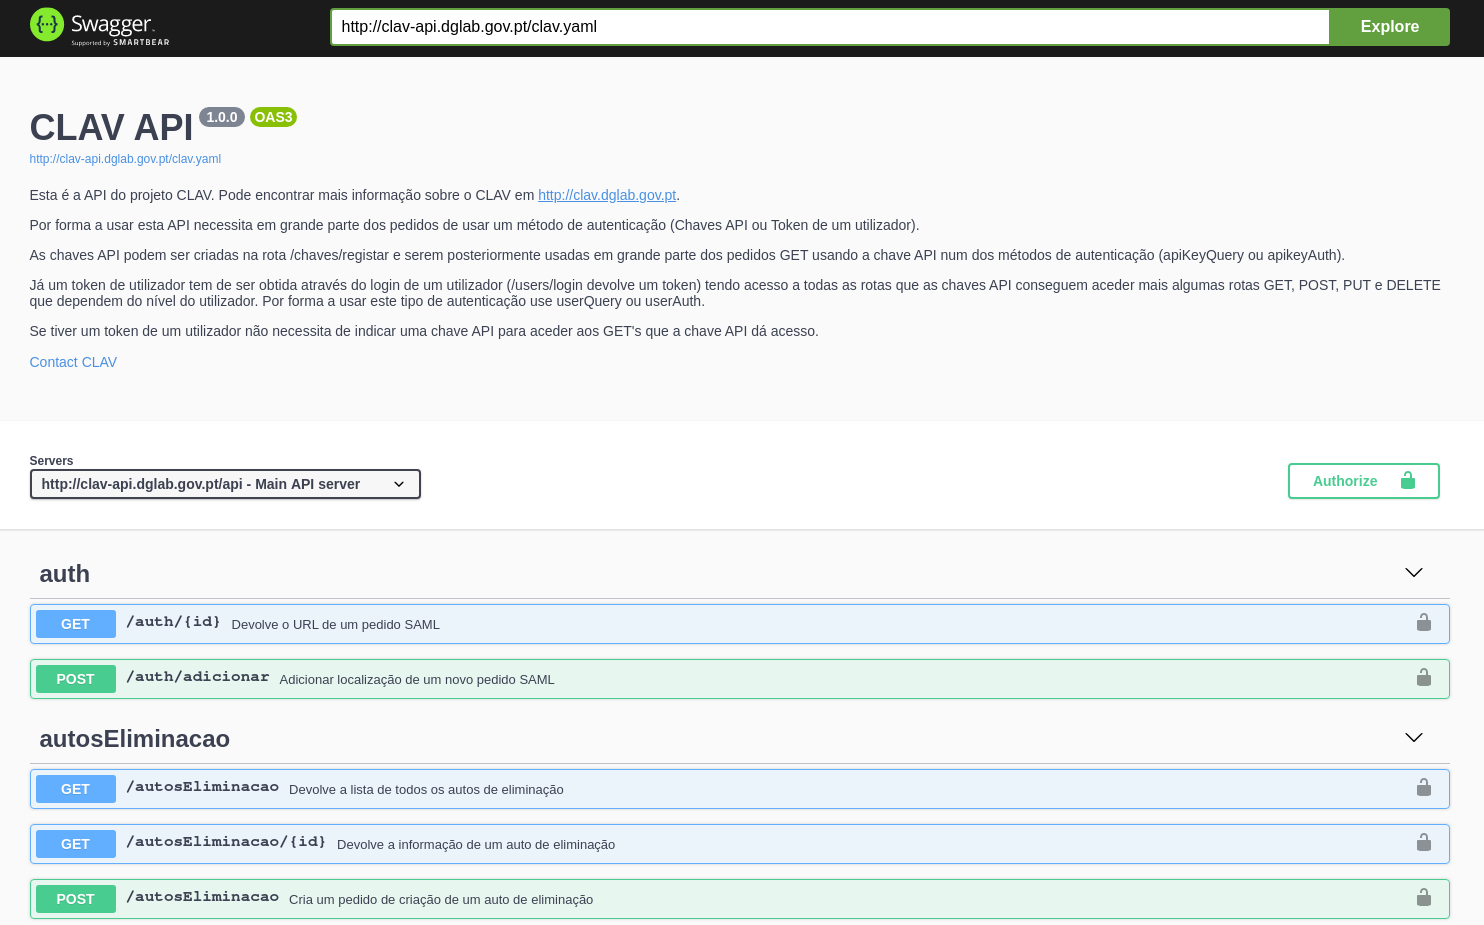
\includegraphics[width=0.7\textwidth]{img/swaggerUI.png}
    \caption{\textit{Swagger \acrshort{ui}} exemplo\label{fig:swaggerUI}}
\end{figure}

\subsubsection{Alternativas}
Existem várias alternativas ao \textit{Swagger \acrshort{ui}}:
\begin{savenotes}
\begin{table}[H]
    \footnotesize
    \centering
    \begin{tabular}{|r|p{0.39\textwidth}|p{0.39\textwidth}|}
    \hline
    Ferramenta & Vantagens & Desvantagens \\ \hline
        \textit{Swagger \acrshort{ui}} &
        \begin{itemize}[leftmargin=0.3cm, topsep=0cm]
            \setlength\itemsep{0em}
            \item Suporta a especificação \textit{OpenAPI}
            \item \textit{Open-source}
            \item Amplamente usado
        \end{itemize}
        &
        %\begin{itemize}[leftmargin=0.3cm, topsep=0cm]
        %    \setlength\itemsep{0em}
        %    \item
        %\end{itemize}
        \\ \hline
    \textit{Apiary}\footnote{Ver \url{https://apiary.io/}} &
        \begin{itemize}[leftmargin=0.3cm, topsep=0cm]
            \setlength\itemsep{0em}
            \item Suporta a especificação \textit{\acrshort{api} Blueprint} e a especificação \textit{OpenAPI}
        \end{itemize}
        &
        \begin{itemize}[leftmargin=0.3cm, topsep=0cm]
            \setlength\itemsep{0em}
            \item Necessário pagar de forma a puder integrar a documentação da \acrshort{api} num domínio próprio
            \item \textit{Closed-source}
        \end{itemize}
        \\ \hline
    \textit{\acrshort{api} Console}\footnote{Ver \url{https://github.com/mulesoft/api-console}} &
        \begin{itemize}[leftmargin=0.3cm, topsep=0cm]
            \setlength\itemsep{0em}
            \item Suporta a especificação \acrshort{raml} e a especificação \textit{OpenAPI}
            \item \textit{Open-source}
        \end{itemize}
        &
        %\begin{itemize}[leftmargin=0.3cm, topsep=0cm]
        %    \setlength\itemsep{0em}
        %    \item
        %\end{itemize}
        \\ \hline
    \textit{Slate}\footnote{Ver \url{https://github.com/slatedocs/slate}} &
        \begin{itemize}[leftmargin=0.3cm, topsep=0cm]
            \setlength\itemsep{0em}
            \item \textit{Open-source}
            \item \acrshort{api} definida em \textit{Markdown}
        \end{itemize}
        &
        \begin{itemize}[leftmargin=0.3cm, topsep=0cm]
            \setlength\itemsep{0em}
            \item Não suporta nenhuma especificação
        \end{itemize}
        \\ \hline
    \textit{apiDoc}\footnote{Ver \url{https://apidocjs.com/}} &
        \begin{itemize}[leftmargin=0.3cm, topsep=0cm]
            \setlength\itemsep{0em}
            \item Documentação criada a partir das anotações nos comentários do código
            \item \textit{Open-source} 
        \end{itemize}
        &
        \begin{itemize}[leftmargin=0.3cm, topsep=0cm]
            \setlength\itemsep{0em}
            \item Não suporta nenhuma especificação
        \end{itemize}
        \\ \hline
    \textit{ReDoc}\footnote{Ver \url{https://github.com/Redocly/redoc}} &
        \begin{itemize}[leftmargin=0.3cm, topsep=0cm]
            \setlength\itemsep{0em}
            \item Suporta a especificação \textit{OpenAPI}
            \item \textit{Open-source} 
            \item Fácil de integrar
        \end{itemize}
        &
        %\begin{itemize}[leftmargin=0.3cm, topsep=0cm]
        %    \setlength\itemsep{0em}
        %    \item
        %\end{itemize}
        \\ \hline
    \end{tabular}
    \caption{Comparação entre ferramentas de \acrshort{api}s}
    \label{table:swaggerUI}
\end{table}
\end{savenotes}

\subsection{Produção da documentação da \glsentryshort{api} da \glsentryshort{clav}}\label{sec:soaDocAPI}

Neste secção são aprofundadas algumas bibliotecas que podem ser usadas para a produção da documentação com a 
especificação \textit{OpenAPI} e o \textit{Swagger \acrshort{ui}}. 

De seguida, são aprofundadas duas \textit{packages} que podem ser usadas para criar documentação 
interativa (integração do \textit{Swagger UI}) para uma \acrshort{api} \acrshort{rest} criada com 
\textit{Node.js} e \textit{Express.js}:~\cite{swaggerNode}
\begin{itemize}
    \item \texttt{swagger-node-express}
    \begin{itemize}
        \item Vantagens
        \begin{itemize}
            \item Módulo oficial suportado pelo \textit{Swagger};
            \item É \textit{open-source} e como tal é possível contribuir para a correção de problemas;
            \item A solução contém \textit{Swagger Editor} e \textit{Swagger Codegen} e como tal tanto 
            podemos usar uma abordagem \textit{top-down} como \textit{bottom-up}.
        \end{itemize}
        \item Desvantagens
        \begin{itemize}
            \item Instalação manual do \textit{Swagger \acrshort{ui}}. O código do \textit{Swagger \acrshort{ui}} 
            tem de ser copiado manualmente para o projeto e sempre que há uma atualização é necessário copiar 
            novamente manualmente;
            \item Instalação complexa. Por forma a aplicação hospedar a documentação é necessário adicionar 
            algumas rotas ao servidor para além das já definidas na especificação \textit{OpenAPI};
            \item Fraca documentação.
        \end{itemize}
    \end{itemize}
    \item \texttt{swagger-ui-express}
    \begin{itemize}
        \item Vantagens
        \begin{itemize}
            \item É \textit{open-source} e como tal é possível contribuir para a correção de problemas;
            \item Não é necessário copiar manualmente o \textit{Swagger \acrshort{ui}};
            \item De fácil instalação, apenas é necessário adicionar uma rota aonde estará hospedada a documentação;
            \item Boa documentação.
        \end{itemize}
        \item Desvantagens
        \begin{itemize}
            \item Não é o módulo oficial suportado pelo \textit{Swagger}.
        \end{itemize}
    \end{itemize}
\end{itemize}

Das duas, a \texttt{swagger-ui-express} é a de mais simples implementação e de mais fácil manutenção.

\begin{lstlisting}[language=javascript, caption=Exemplo de uso do \texttt{swagger-ui-express}, label=exem:suie]
var swaggerUI = require('swagger-ui-express')
//JSON
var swaggerDocument = require('./swagger.json')
//ou YAML
var yaml = require('js-yaml')
var fs = require('fs')
var swaggerDocument = yaml.load(fs.readFileSync('./swagger.yaml'))

app.use('/doc', swaggerUI.serve, swaggerUI.setup(swaggerDocument));
\end{lstlisting}

No exemplo~\ref{exem:suie} a documentação da \acrshort{api} está presente na rota \texttt{'/doc'}. 
Neste exemplo percebe-se como carregar uma especificação \textit{OpenAPI} em \acrshort{json} bem como 
em \acrshort{yaml}. Quanto ao \textit{middleware} \texttt{serve} retorna os ficheiros estáticos necessários 
para hospedar o \textit{Swagger \acrshort{ui}}. Já o segundo \textit{middleware} \texttt{setup} para além de 
poder receber o documento com a especificação \textit{OpenAPI} pode também receber um outro parâmetro de opções 
que o utilizador pode definir para a apresentação interativa da documentação com o 
\textit{Swagger \acrshort{ui}}\footnote{As opções possíveis estão presentes em \url{https://github.com/scottie1984/swagger-ui-express}. Para o atributo (opção) \texttt{swaggerOptions} as opções possíveis estão presentes em \url{https://github.com/swagger-api/swagger-ui/blob/master/docs/usage/configuration.md}}.

Agora há duas abordagens possíveis de realizar a documentação:
\begin{itemize}
    \item Documentação de cada rota nos comentários da rota através da utilização da 
    \textit{package} \texttt{swagger-jsdoc}\footnote{Ver \url{https://github.com/Surnet/swagger-jsdoc}};
    \item Documentação à parte do código.
\end{itemize}

A abordagem da documentação à parte do código permite modularizar a documentação. A modularização da documentação 
pode ser realizada através do uso da \textit{package} \texttt{yaml-include}\footnote{Ver \url{https://github.com/claylo/yaml-include}}. Esta \textit{package} permite que o documento \acrshort{yaml} da especificação \textit{OpenAPI} possa ser dividida por vários ficheiros para além do que já é permitido através do uso de \verb|$ref| da especificação \textit{OpenAPI}. A \textit{package} permite a inclusão de arquivos \acrshort{yaml} externos ou a inclusão de pastas de ficheiros \acrshort{yaml}. Esta funcionalidade é desaprovada pela equipa de desenvolvimento do \acrshort{yaml} contudo ajuda e simplifica a construção do ficheiro de especificação \textit{OpenAPI}.

\begin{lstlisting}[language=yaml, caption=Exemplo de uso do \texttt{yaml-include} no documento de especificação \textit{OpenAPI}(\textit{index.yaml}), label=exem:yamli]
openapi: 3.0.0
info:
  description: Esta é a API do projeto CLAV. Pode encontrar mais informação sobre o CLAV em [http://clav.dglab.gov.pt](http://clav.dglab.gov.pt).
  version: 1.0.0
  title: CLAV API
  contact:
    name: CLAV
    email: clav@dglab.gov.pt
servers:
  - url: http://localhost:7779/api
    description: Local API server
paths: !!inc/dir [ 'paths' ]
components:
  schemas: !!inc/dir [ 'schemas', excludeTopLevelDirSeparator: true ]
  securitySchemes: !!inc/file '/security/schemes.yaml'
\end{lstlisting}

O ficheiro \textit{index.yaml} será a raiz do documento de especificação \textit{OpenAPI} a ser gerado com 
a \textit{package} \texttt{yaml-include}. A seguinte estrutura dos ficheiros exemplifica como se pode dividir a 
documentação por vários ficheiros com esta \textit{package} para gerar o documento de especificação \textit{OpenAPI}:
\begin{lstlisting}[caption=Exemplo de estrutura dos ficheiros para gerar o documento de especificação \textit{OpenAPI}, label=exem:faf]
* index.yaml
* paths/
    * classes/
        * get.yaml
        * ~id/
            * get.yaml
    * users/
        * ~id/
            * post.yaml
            * delete.yaml
* schemas/
    * User.yaml
* security/
    * schemes.yaml
\end{lstlisting}

Assim, o \texttt{!!inc/dir} fará com que no ficheiro \textit{index.yaml} na \textit{tag} \textit{paths} sejam 
incluídos todos os ficheiros que estão na pasta \textit{paths}. Cada ficheiro corresponderá a uma determinada 
rota com um determinado método \acrshort{http}. O método \acrshort{http} é definido a partir do nome do ficheiro 
e o caminho da rota é determinado pelo nome das pastas e do aninhamento destas. Quando o nome da pasta é iniciado 
por ``\verb|~|'' no caminho será colocado o nome da pasta sem o til e entre chavetas (``\{\}'') por forma a 
indicar um parâmetro que é colocado no caminho do pedido.

Já no caso do \texttt{!!inc/dir} dos \textit{schemas} a opção \texttt{excludeTopLevelDirSeparator} permite que 
os ficheiros que estejam dentro da pasta \textit{schemas} (mas não aninhados dentro de outras pastas) sejam 
incluídos sem qualquer aninhamento, assumindo o nome do ficheiro como o atributo a colocar.

Existe também o \texttt{!!inc/file} que permite incluir sobe uma determinada \textit{tag} a informação presente 
no ficheiro referenciado pelo caminho.

O documento de especificação \textit{OpenAPI} final gerado será:
\begin{lstlisting}[language=yaml, caption=Documento de especificação \textit{OpenAPI} gerado a partir do ficheiro \textit{index.yaml} com o uso da \textit{package} \texttt{yaml-include}, label=exem:yamlif]
openapi: 3.0.0
info:
  description: Esta é a API do projeto CLAV. Pode encontrar mais informação sobre o CLAV em [http://clav.dglab.gov.pt](http://clav.dglab.gov.pt).
  version: 1.0.0
  title: CLAV API
  contact:
    name: CLAV
    email: clav@dglab.gov.pt
servers:
  - url: http://localhost:7779/api
    description: Local API server
paths:
  /classes:
    get:
      <conteúdo do ficheiro paths/classes/get.yaml>
  /classes/{id}:
    get:
      <conteúdo do ficheiro paths/classes/~id/get.yaml>
  /users/{id}:
    post:
      <conteúdo do ficheiro paths/users/~id/post.yaml>
    delete:
      <conteúdo do ficheiro paths/users/~id/delete.yaml>
components:
  schemas:
    User:
      <conteúdo do ficheiro schemas/User.yaml>
  securitySchemes:
    <conteúdo do ficheiro security/schemes.yaml>
\end{lstlisting}

No final teremos um ficheiro no formato \acrshort{yaml} com toda a documentação da \acrshort{api} que puderá 
então ser usado para alimentar a documentação dinâmica \textit{Swagger \acrshort{ui}}.

\section{Solução}

No estado da arte foram abordadas várias alternativas ao \textit{Swagger UI}. 
A partir da tabela~\ref{table:swaggerUI} e tendo em conta que:
\begin{itemize}
    \item Não há financiamento;
    \item Já existe uma \acrshort{api} desenvolvida;
    \item A documentação deve estar acessível de um domínio próprio;
    \item A documentação deve ser fácil de criar, de editar e de manter;
    \item Será usada a especificação \textit{OpenAPI}.
\end{itemize}

As várias alternativas ficam reduzidas ao \textit{Swagger \acrshort{ui}} e ao \textit{ReDoc}. 
Optou-se por escolher o \textit{Swagger \acrshort{ui}} visto ser a ferramenta mais amplamente usada para além de 
que é possível obter também uma fácil integração no \textit{Swagger \acrshort{ui}} com recurso 
à \textit{package} \texttt{swagger-ui-express} já aprofundada no estado da arte (ver~\ref{sec:soaDocAPI}). 
Além disso, escolheu-se a \textit{package} \texttt{yaml-include} por forma a auxiliar a produção da 
documentação na criação do ficheiro com a especificação \textit{OpenAPI}, permitindo que esta documentação 
seja modular.

A documentação modular será estruturada da seguinte forma:

\begin{lstlisting}[caption=Excerto da estrutura modular da documentação]
* /index.yaml
* /paths/
    * /classes/
        * /get.yaml
        * /post.yaml
        * /~id/
            * /get.yaml
            ...
        ...
    ...
* /examples/
    * /classes/
        * /ClasseCompletaJSON.yaml
        * /ClasseCompletaXML.yaml
        * /ClasseSimplesJSON.yaml
        ...
    ...
* /schemas/
    * /classes/
        * /ClasseCompleta.yaml
        ...
    * /definicoes/
        * Codigo.yaml
        ...
    ...
\end{lstlisting}

Portanto nesta estrutura na pasta \texttt{paths} é seguida a estrutura do \texttt{yaml-include} já descrita no 
estado da arte em~\ref{exem:faf} em que as pastas indicam o caminho e o nome dos ficheiros o verbo \acrshort{http} 
da rota. Em cada um destes ficheiros é colocada a descrição, os parâmetros, etc, da rota. 
Nestes ficheiros serão feitas referências aos \texttt{schemas} e \texttt{examples} necessários, estando estes nas 
pastas \texttt{schemas} e \texttt{examples} respetivamente. Isto permite que os modelos e os exemplos sejam 
reutilizados para além de que permite tornar os ficheiros onde são referenciados mais fáceis de perceber, 
principalmente nos casos em que os modelos e os exemplos são extensos.

Em termos de organização das pastas \texttt{schemas} e \texttt{examples}, estas no primeiro ``nível'' possuem 
pastas de cada grupo de rotas (classes, entidades, \textit{users}, chaves, etc) e em cada uma destas pastas estão 
os modelos/exemplos correspondentes a esse grupo de rotas. Na pasta \texttt{schemas} existe contudo uma pasta 
especial chamada \texttt{definicoes} que possui os vários tipos de dados, como por exemplo o código de uma classe, 
o id de uma entidade, etc. Assim, estes modelos são usados nos outros modelos e nas rotas permitindo uniformizar 
estes dados. Ou seja, caso haja por exemplo alguma alteração no formato do código, será apenas necessário alterar 
no modelo presente na pasta \texttt{definicoes} que a alteração será ``propagada'' já que todos que precisam deste 
modelo incluem-no por referência. 

Portanto, sempre que é criado um novo modelo ou uma nova rota, convém verificar nesta pasta \texttt{definicoes} 
se já existe o tipo de dados necessário a usar bastando assim fazer-lhe referência.

Por fim, no ficheiro \texttt{index.yaml} são definidos os grupos de rotas (\textit{tags}) bem como várias 
informações gerais sobre a \acrshort{api} de dados, como descrição, métodos de autenticação, etc. 
Além disso, é aqui também definido, apenas no caso da pasta \texttt{examples}, que ficheiros deve o 
\texttt{yaml-include} ignorar ao incluir a pasta \texttt{examples} sobre a \textit{tag} \texttt{examples} 
dos \texttt{components}. Isto é efetuado por forma a evitar erros de sintaxe da especificação \textit{OpenAPI}. 
Estes erros acontecem porque há vários ficheiros de exemplos a serem incluídos nos ficheiros das rotas diretamente 
pelo \texttt{yaml-include} em vez de se usar o \verb|$ref| da especificação \textit{OpenAPI} em casos que o 
\verb|$ref| não permite efetuar o pretendido. Assim, estes ficheiros têm de ser ignorados.

Com o \texttt{yaml-include}, sempre que a \acrshort{api} de dados inicia é criado o ficheiro de especificação 
\textit{OpenAPI} final que incluirá os dados destes ficheiros nos seus locais apropriados. 
Este ficheiro final ficará disponível na pasta pública do servidor com o nome \texttt{clav.yaml} 
ou seja acessível a partir de \url{https://clav-api.dglab.gov.pt/clav.yaml}. É este o ficheiro que alimenta o 
\textit{SwaggerUI} construído com o \textit{swagger-ui-express} e disponível em 
\url{https://clav-api.dglab.gov.pt/v2/docs}.

\section{Implementação}

A documentação da \acrshort{api} de dados da \acrshort{clav} já se encontra disponível em \url{https://clav-api.dglab.gov.pt/v2/docs}, possuindo uma descrição inicial de como os utilizadores podem obter \textit{tokens} e usar a \acrshort{api} de dados a partir do \textit{Swagger UI}. Esta documentação em cada rota possui uma descrição, \textit{query strings} que podem ser definidas, exemplos de \textit{bodies} quando aplicável, possíveis respostas bem como exemplos de respostas. Além disso, tanto os \textit{bodies} e as respostas quando possuem exemplos possuem também o esquema desse \textit{body}/resposta.

Para experimentar uma rota, é então apenas necessário selecionar uma rota, carregar em \textit{Try it out}, inserir os valores que pretende e carregar em \textit{Execute}. Isto claro sem a autenticação. Com autenticação, após obter o \textit{token} para o usar deve carregar no cadeado aberto, selecionar a forma de colocar o \textit{token} no pedido que pretende: 
\begin{itemize}
    \item para Chaves \acrshort{api}:
    \begin{itemize}
        \item Na \textit{query string}: \texttt{apiKeyQuery}
        \item No cabeçalho \texttt{Authorization}: \texttt{apiKeyAuth}
    \end{itemize}
    \item para Utilizadores:
    \begin{itemize}
        \item Na \textit{query string}: \texttt{userQuery}
        \item No cabeçalho \texttt{Authorization}: \texttt{userAuth}
    \end{itemize}
\end{itemize}
inserir o \textit{token} corretamente (atenção que os casos em que é inserido no cabeçalho \texttt{Authorization} são especiais), carregar em \textit{Authorize} e depois já poderá aceder às rotas. Ao efetuar este passo uma vez, o \textit{Swagger UI} usa o mesmo \textit{token} nas restantes rotas que possui a mesma forma de autenticação não necessitando deste passo nessas (aquelas em que o cadeado se encontra fechado).

\section{Resumo}

Resumidamente, após entender a especificação \textit{OpenAPI}, o \textit{Swagger UI} e possível abordagem de escrita no estado da arte deste capítulo,
descreveu-se na secção solução como a documentação é escrita e apresentada ao utilizador. 

Por fim, na secção da implementação descreveu-se de que forma pode ser usada esta documentação já disponível em \url{https://clav-api.dglab.gov.pt/v2/docs}.
